\section{ICBA and Two Recovery Policies}
\label{sec:auditor}

\subsection{The Audit Contract}
ICBA leaves graph construction and native traversal unchanged. Its input contract names the source and target snapshots, implementation, query population, action grid, permitted observations, failure event, and reference policy. Its output records raw reuse, the selected action, certification counts and bounds, actual fallback, execution risk, and lifecycle cost. These fields also expose when two experimental settings cannot be quantitatively combined.

Target information has three separate uses. Selection chooses a policy using its assigned queries. Certification checks that frozen policy and any fallback; it does not retrain or reorder them. Evaluation measures the completed decision, including fallback executions. A raw-reuse row is retained even if it would fail certification, so a successful endpoint cannot hide an unsuccessful transferred policy. If no policy qualifies, the audit outputs abstention; diagnostic endpoint execution is recorded as unqualified, not approved deployment.

\subsection{TCP: History Pooling Followed by One Target Shift}
\label{sec:tcp-implementation}
The recovery experiment uses native HNSW actions
\begin{equation}
 \mathcal A=(10,20,40,80,120,160,200).\label{eq:tcp-grid}
\end{equation}
For each query and old build, encode the first-passing grid index as $\tilde j_g(q)$; if none passes, store $J$ while retaining the unresolved flag. For target seed $t$, pool the nine old builds other than the matched seed:
\begin{equation}
 j_0^{(t)}(q)=\max_{g\in\mathcal H_t}\tilde j_g(q),\qquad
 \pi_s(q)=a_{\min\{j_0^{(t)}(q)+s,J\}}.\label{eq:shift}
\end{equation}
The same-query old profiles exist for all three target roles. Thus TCP operates on a recurring, profiled workload, not unseen-query budget prediction. Storing a pooled index costs $O(Q)$ for $Q$ profiles; a serving decision is a lookup, addition, and clipping before native search. Acquiring those profiles is a separate, potentially dominant expense.

Target selection scans $s=0,\ldots,J-1$ in ascending order and takes the first shift whose selection-role CP bound at $\alpha=0.05$ is at most 0.05. If none passes, it returns the endpoint shift. This is a selection heuristic, not a multiple-testing certificate or a minimum-NDC optimizer. Both the selected policy and the endpoint are then fixed before certification.

The acronym TCP is retained from the project's history-pooling family; in this paper it denotes the \emph{target-calibrated pooling replay} just defined. Historical artifacts call that family Tiered Conformal Pooling and include a different stable-tail variant at $\tau=0.90$. That variant is not substituted for the first-passing, $\tau=0.95$ results here. The name does not import the exchangeable-build assumptions of Equation~\eqref{eq:pooling}.

\subsection{Original Decisions and a Joint-Error Sensitivity}
\label{sec:tcp-recalibration}
The original replay checks the selected candidate and endpoint separately at $\alpha=0.05$ each. It accepts the candidate if its bound passes, otherwise executes the endpoint with the endpoint's qualification flag. The two allocations sum to 0.10, so they do not provide a 95\% guarantee for the combined selection procedure.

We therefore add a \emph{post-hoc frozen-response sensitivity}: keep every selected shift unchanged, use $\alpha_c=\alpha_e=0.025$, and apply the same candidate-first order. If neither policy passes, abstain. This instantiates Proposition~\ref{prop:simultaneous} at total $\alpha=0.05$ under its query-sampling assumptions, separately for each target. It does not rerun selection, enlarge the action class, or use evaluation to choose a new threshold. Its results are reported alongside the original decisions, not presented as a preregistered replication.

Figure~\ref{fig:workflow} shows the data flow. The audit is reusable independently of TCP: a learned termination rule or a fixed budget can occupy the candidate input, provided its observation contract and failure event are retained.
\begin{figure*}[t]
\centering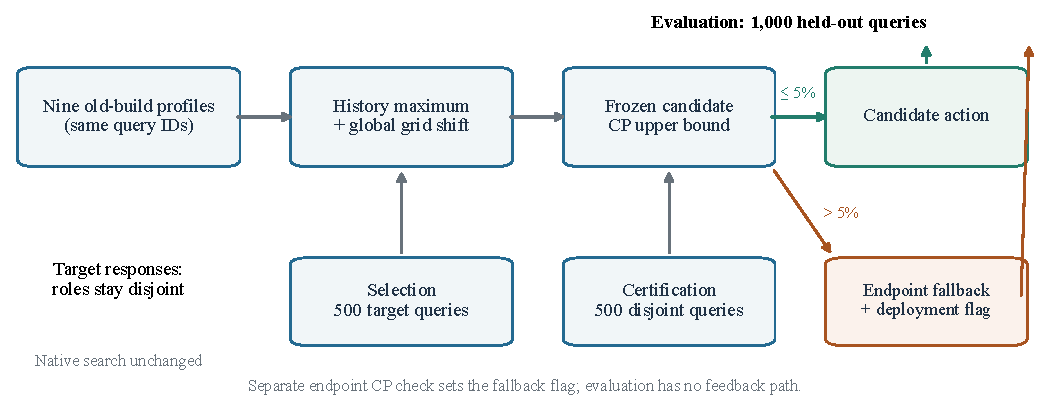
\includegraphics[width=\textwidth]{figures/workflow.pdf}
\caption{ICBA applied to TCP. Same-query old-build profiles define the pooled policy for each target role. Selection chooses one global shift; certification checks the frozen candidate and endpoint; evaluation has no feedback path. The original replay assigns 0.05 to each check. The joint-error sensitivity assigns 0.025 to each, allowing a per-target union bound of 0.05.}
\label{fig:workflow}
\Description{Historical profiles feed an ordered shift selected on 500 queries. A separate 500-query certification role chooses candidate, endpoint, or abstention. Another 1,000 queries evaluate the selected decision.}
\end{figure*}

\subsection{A Source-Certified Slack Bridge}
\label{sec:slack-method}
The second recovery policy removes TCP's target-selection step. For each source build, a source-only design role fixes an action $a_s$. Three registered lanes execute $a_s$ shifted upward by zero, one, or two native grid levels, clipped at the endpoint. On 500 previously untouched source-certification queries, each lane and its endpoint receive error allocations $\alpha_c=\alpha_e=0.025$. A lane is deployable for that source only when both bounds are at most $\delta=0.05$; otherwise it falls back to the certified endpoint. Another 500 untouched queries evaluate the frozen source-to-target decision over all non-diagonal build pairs.

This bridge uses no target selection, target labels, retrospective stable-tail action, or evaluation feedback. The three lanes are separate preregistered estimands rather than a best-after-observation search. Consequently, the experiment can show that a particular fixed slack transfers within a registered implementation family, but not that the lane is uniformly optimal or jointly selected at 95\% confidence across implementations.
